%sensory systems generally
The sensory systems of brains do remarkable work in extracting behaviorally useful information from noisy and complex raw sense data. 
Vision systems process intensities from retinal photoreceptor arrays, auditory systems interpret the amplitudes and frequencies of hair-cell displacements, and somatosensory systems integrate data from direct physical interactions.~\cite{purves2001neuroscience} 
Although these systems differ radically in their input modalities, total number of neurons, and specific neuronal microcircuits, they share two fundamental characteristics. 
First, they are hierarchical sensory cascades, albeit with extensive feedback, consisting of sequential processing stages that together produce a complex transformation of the input data.  
Second, they operate in inherently highly-structured spatiotemporal domains, and are generally organized in maps that reflect this structure~\cite{felleman1991distributed}.

Extensive experimental work in the rodent whisker-trigeminal system has provided insights into how these principles help rodents use their whiskers (also known as \emph{vibrissae}) to tactually explore objects in their environment.  
Similar to hierarchical processing in the visual system (e.g., from V1 to V2, V4 and IT~\cite{felleman1991distributed, Goodale1992}), processing in the somatosensory system is also known to be hierarchical\cite{Pons1987, Inui2004, Iwamura1998}.  
For example, in the whisker trigeminal system, information from the whiskers is relayed from primary sensory neurons in the trigeminal ganglion to multiple trigeminal nuclei~\cite{}. The trigeminal nuclei are the origin of several parallel pathways conveying information to the thalamus and then primary and secondary somatosensory cortex (S1 and S2)~\cite.  
However, although the rodent somatosensory system has been the subject of extensive experimental efforts\cite{armstrong1992flow, petersen2003spatiotemporal, kerr2007spatial, von2007neuronal}, there have been comparatively few attempts at computational modeling of this important sensory system. 

\begin{figure}
\centering
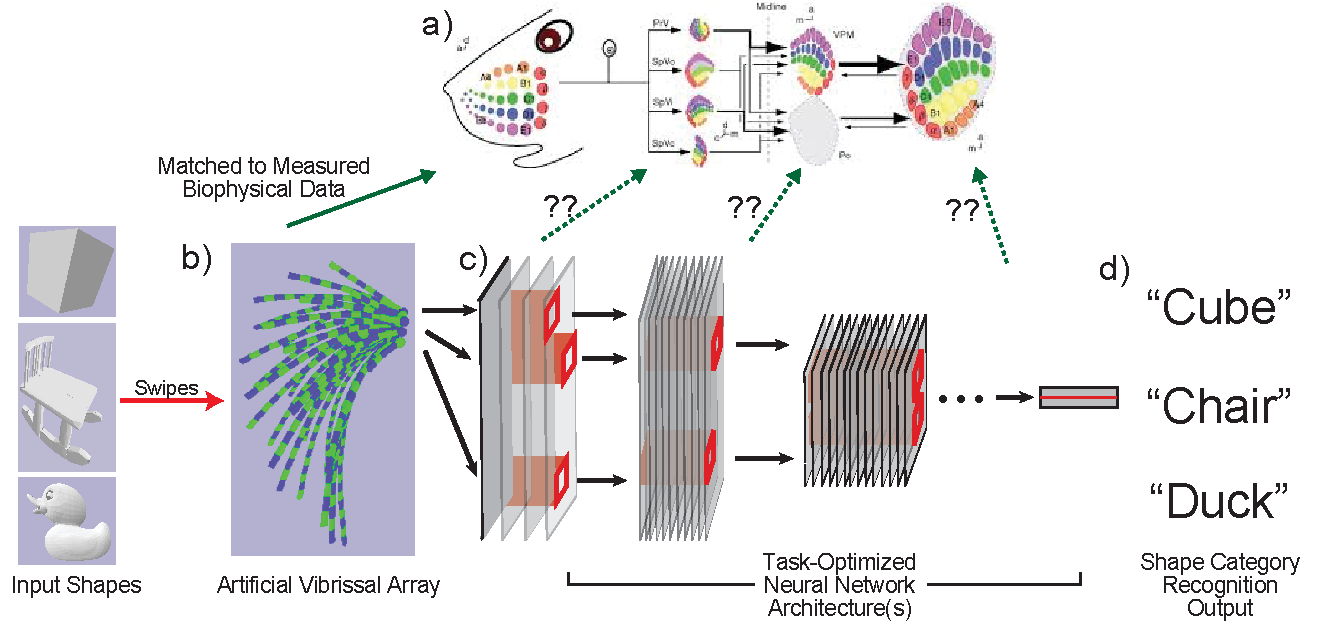
\includegraphics[width=.85\linewidth]{figures/schematic.pdf}
\vspace{-3mm}
\caption{\footnotesize{\textbf{Goal-Driven Approach to Modeling Barrel Cortex:} \textbf{a.} Rodents have highly sensitive whisker (vibrissal) arrays that provide input data about the environment. Mechanical signals from the vibrissae are relayed by primary sensory neurons of the trigeminal ganglion to the trigeminal nuclei, the original of multiple parallel pathways to S1 and S2.  This system is a prime target for modeling because it is likely to be richly representational, but its computational underpinnings are largely unknown. Our long-term approach to modeling the whisker-trigeminal system is \emph{goal-driven}: using an artificial whisker-array input device built using extensive biophysical measurements (\textbf{b.}), we seek to optimize neural networks of various architectures (\textbf{c.}) to solve ethologically-relevant shape recognition tasks (\textbf{d.}), and then measure to the extent to which these networks predict fine-grained response patterns in real neural recordings.} ~\label{fig_schematic}}
\vspace{-5mm}
\end{figure}

Recent work has shown that deep neural networks (DNNs), whose architectures inherently contain hierarchy and spatial structure, can be effective models of neural processing in vision\cite{Yamins2014,khaligh2014deep} and audition\cite{kell_yamins_sfn}.
Motivated by these successes, in this work we illustrate initial steps toward using DNNs to model rodent somatosensory systems.
Our driving hypothesis is that the vibrissal-trigeminal system is optimized to use whisker-based sensor data to solve somatosensory tasks in complex, variable real-world environments.
The underlying idea of this approach is thus to use \emph{goal-driven} modeling (Fig \ref{fig_schematic}), in which the DNN parameters --- both discrete and continuous --- are optimized for performance on a challenging ethologically-relevant task\cite{yamins2016using}.
Insofar as the shape recognition task is a strong constraint on network parameters, the resulting optimized neural network may be an effective model of real trigeminal-system neural response patterns.

This idea is conceptually straightforward, but implementing it involves surmounting several challenges.
Unlike vision or audition, where signals from the retina or cochlea can for many purposes be approximated by a simple data array (namely, a uniform data array representing light or sound intensities and frequencies), the equivalent mapping from stimulus (e.g. object in a scene) to sensor input in the whisker system is much less direct.
Thus, a biophysically-realistic embodied model of the whisker array is a critical first component of any model of the vibrissal system.
Once the sensor array is available, a second key problem is building a neural network that can accept whisker data input and use it to solve relevant tasks.
Aside from the question of the neural network design itself, knowing what the ``relevant tasks'' are for training a rodent whisker system, in a way that is sufficiently concrete to be practically actionable, is a significant unknown, given the very limited amount of ethologically-relevant behavioral data on rodent sensory capacities\cite{von2007neuronal, Knutsen2006, OConnor2010, Arabzadeh2005, Diamond2008}.
Collecting neural data of sufficient coverage and resolution to quantitatively evaluate one or more task-optimized neural network models represents a third major challenge.
In this work, we show initial steps toward the first two of these problems (sensor modeling and neural network design/training).



